\documentclass[12pt]{beamer}

\usepackage[utf8]{inputenc}
\usepackage{listings,tikz,amsmath,xcolor}

\lstset{language=C++, basicstyle=\footnotesize, frame=single}
\colorlet{mygreen}{green!70!black!50}
\colorlet{myred}{red!60!black!80}
\tikzset{
    every node/.style={draw,thick},
    every path/.style={thick},
    a/.style={rectangle, minimum size=.65cm},
    b/.style={circle, inner sep=0.1cm, minimum size=0.75cm},
    win/.style={fill=mygreen},
    lose/.style={fill=myred,dashed},
    small/.style={scale=0.7, font=\small},
    choice/.style={->, ultra thick},
    pruned/.style={gray,dashed}
}

\beamertemplatenavigationsymbolsempty
\AtBeginSection[]
{
    \begin{frame}
    \frametitle{Table of Contents}
    \tableofcontents[currentsection]
    \end{frame}
}

\title{Game theory}
\subtitle{Nim game, Minimax, Alpha-Beta pruning}
\author{beOI Training}
\institute{
\includegraphics[height=12em]{../share/beoi-logo}}

\begin{document}

\maketitle


\section{Basics and game trees}
\begin{frame}
\frametitle{What is game theory?}
Modelling strategic situations:
\begin{itemize}
\item with conflict or cooperation
\begin{itemize} \item chess, football, pictionary, ... \end{itemize}
\item decisions based on personal goals
\begin{itemize} \item beating the opponent, maximizing points, ... \end{itemize}
\item influenced by the choice patterns of other players
\begin{itemize} \item if someone plays predictably, you can use it against them \end{itemize}
\item might involve randomness
\begin{itemize} \item dice rolls, card draws, ... \end{itemize}
\end{itemize}

~

Goal: compute choices, optimal strategies, expected gains
\end{frame}

\begin{frame}
\frametitle{Game trees}
A useful tool to examine decisions and their consequences.
\begin{center}
\includegraphics[width=.95\linewidth]{img/tictactoe}
\end{center}
\end{frame}

\begin{frame}
\frametitle{Utility vectors and zero-sum games}
Utility vectors:
\begin{itemize}
\item define the ``gains'' of an end state
\item one entry per player: $(2,3,-2)$, $(0,7)$, ...
\item determine the choices of players
\begin{itemize} \item player 1 will choose $({\bf 3},5)$ over $({\bf 2},3)$ \end{itemize}
\item but not always!
\begin{itemize} \item should player 2 choose $(0,{\bf 6},5)$ or $(2,{\bf 6},3)$? \end{itemize}
\end{itemize}

~

Main focus: two-player zero-sum games:
\begin{itemize}
\item only two players: no complicated interactions
\item zero-sum: our benefits are the opponent's losses
\begin{itemize} \item $(5,-5)$, $(-3,3)$, $(0,0)$, ... (or just $5$, $-3$, $0$) \end{itemize}
\item the value of a choice is always well-defined
\end{itemize}
\end{frame}


\section{Bachet's game}
\begin{frame}
\frametitle{Bachet's game: rules}
``Jeu des alumettes'' in French, ??? in Dutch
\begin{itemize}
\item At the beginning, $n$ matches on the table
\item Two players play in alternance
\item At each turn they remove $1,2,\ldots,k$ matches
\item The player that takes the last match wins
\end{itemize}

~

Example with $k=3$:
\begin{itemize}
\item At the beginning, $n = 8$ matches.
\item Player A takes 2; remaining: 6.
\item Player B takes 2; remaining: 4.
\item Player A takes 3; remaining: 1.
\item Player B takes 1 and wins.
\end{itemize}
\end{frame}

\begin{frame}
\frametitle{Bachet's game: game tree}
\tikz{\node[a, small, label=right:{\ = A plays}] {?};}
\quad
\tikz{\node[b, small, label=right:{\ = B plays}] {?};}

\begin{center}
\scalebox{0.9}{
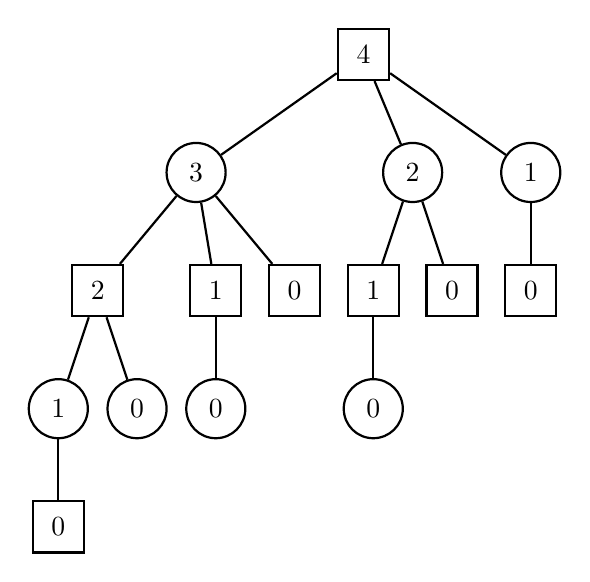
\begin{tikzpicture}

\node[a] at (3.875,6) (n00) {4};

\node[b] at (1.75,4.5) (n10) {3};
\node[b] at (4.5,4.5) (n11) {2};
\node[b] at (6,4.5) (n12) {1};

\node[a] at (.5,3) (n20) {2};
\node[a] at (2,3) (n21) {1};
\node[a] at (3,3) (n22) {0};
\node[a] at (4,3) (n23) {1};
\node[a] at (5,3) (n24) {0};
\node[a] at (6,3) (n25) {0};

\node[b] at (0,1.5) (n30) {1};
\node[b] at (1,1.5) (n31) {0};
\node[b] at (2,1.5) (n32) {0};
\node[b] at (4,1.5) (n33) {0};

\node[a] at (0,0) (n40) {0};

\draw (n00) -- (n10);
\draw (n00) -- (n11);
\draw (n00) -- (n12);

\draw (n10) -- (n20);
\draw (n10) -- (n21);
\draw (n10) -- (n22);
\draw (n11) -- (n23);
\draw (n11) -- (n24);
\draw (n12) -- (n25);

\draw (n20) -- (n30);
\draw (n20) -- (n31);
\draw (n21) -- (n32);
\draw (n23) -- (n33);

\draw (n30) -- (n40);
\end{tikzpicture}
}
\end{center}
\end{frame}

\begin{frame}
\frametitle{Winning states}
\begin{itemize}
\item A winning state is a state such that the \emph{current player} has winning strategy
\item A state is winning iff one of the moves leads to a losing state for the opponent
\item If all the next states are winning for the opponent, then we can't win!
\end{itemize}

~

\tikz{\node[a, win, small, label=right:{\ = winning}] {?};}
\quad
\tikz{\node[a, lose, small, label=right:{\ = losing}] {?};}
\quad
\tikz{
    \node[a, small, label=right:{\ = choice}] (a) {?};
    \draw[choice] (-0.8,0) -- (a);
}

\begin{center}
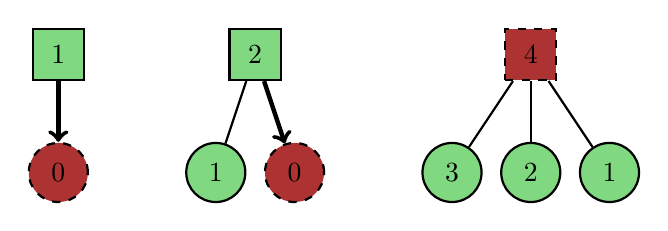
\begin{tikzpicture}
\node[a,win] at (0,1.5) (a1) {1};
\node[b,lose] at (0,0) (a0) {0};
\draw[choice] (a1) -- (a0);

\node[a,win] at (2.5,1.5) (b2) {2};
\node[b,win] at (2,0) (b1) {1};
\node[b,lose] at (3,0) (b0) {0};
\draw (b2) -- (b1);
\draw[choice] (b2) -- (b0);

\node[a,lose] at (6,1.5) (c4) {4};
\node[b,win] at (5,0) (c3) {3};
\node[b,win] at (6,0) (c2) {2};
\node[b,win] at (7,0) (c1) {1};
\draw (c4) -- (c3);
\draw (c4) -- (c2);
\draw (c4) -- (c1);
\end{tikzpicture}
\end{center}
\end{frame}

\begin{frame}
\frametitle{Bachet's game: winning states}
\begin{center}
\scalebox{0.65}{
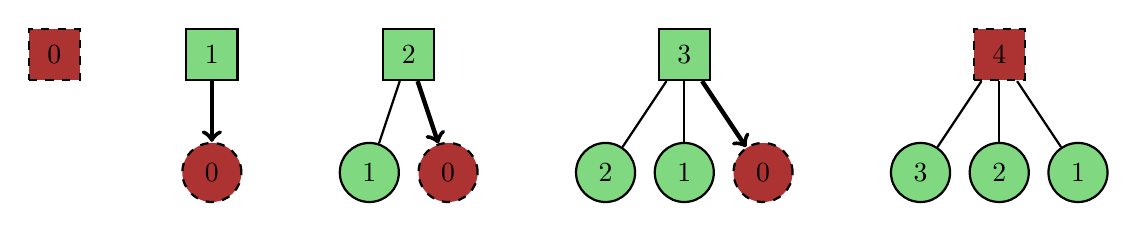
\begin{tikzpicture}
\node[a,lose] at (-2,1.5) {0};

\node[a,win] at (0,1.5) (a1) {1};
\node[b,lose] at (0,0) (a0) {0};
\draw[choice] (a1) -- (a0);

\node[a,win] at (2.5,1.5) (b2) {2};
\node[b,win] at (2,0) (b1) {1};
\node[b,lose] at (3,0) (b0) {0};
\draw (b2) -- (b1);
\draw[choice] (b2) -- (b0);

\node[a,win] at (6,1.5) (c3) {3};
\node[b,win] at (5,0) (c2) {2};
\node[b,win] at (6,0) (c1) {1};
\node[b,lose] at (7,0) (c0) {0};
\draw (c3) -- (c2);
\draw (c3) -- (c1);
\draw [choice] (c3) -- (c0);

\node[a,lose] at (10,1.5) (d4) {4};
\node[b,win] at (9,0) (d3) {3};
\node[b,win] at (10,0) (d2) {2};
\node[b,win] at (11,0) (d1) {1};
\draw (d4) -- (d3);
\draw (d4) -- (d2);
\draw (d4) -- (d1);
\end{tikzpicture}
}

~

\scalebox{0.65}{
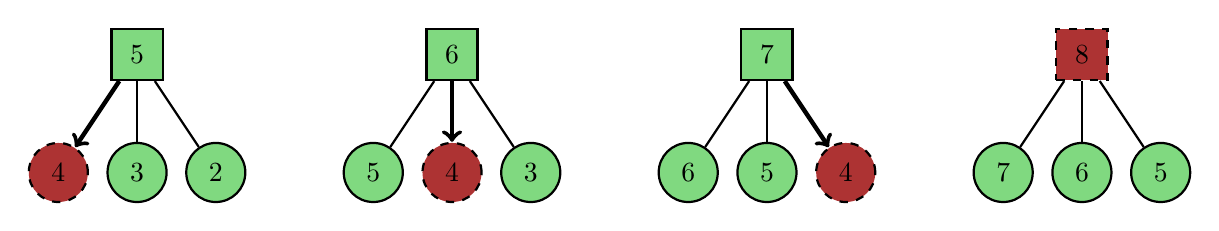
\begin{tikzpicture}
\node[a,win] at (1,1.5) (a5) {5};
\node[b,lose] at (0,0) (a4) {4};
\node[b,win] at (1,0) (a3) {3};
\node[b,win] at (2,0) (a2) {2};
\draw [choice] (a5) -- (a4);
\draw (a5) -- (a3);
\draw (a5) -- (a2);

\node[a,win] at (5,1.5) (b6) {6};
\node[b,win] at (4,0) (b5) {5};
\node[b,lose] at (5,0) (b4) {4};
\node[b,win] at (6,0) (b3) {3};
\draw (b6) -- (b5);
\draw [choice] (b6) -- (b4);
\draw (b6) -- (b3);

\node[a,win] at (9,1.5) (c7) {7};
\node[b,win] at (8,0) (c6) {6};
\node[b,win] at (9,0) (c5) {5};
\node[b,lose] at (10,0) (c4) {4};
\draw (c7) -- (c6);
\draw (c7) -- (c5);
\draw [choice] (c7) -- (c4);

\node[a,lose] at (13,1.5) (d8) {8};
\node[b,win] at (12,0) (d7) {7};
\node[b,win] at (13,0) (d6) {6};
\node[b,win] at (14,0) (d5) {5};
\draw (d8) -- (d7);
\draw (d8) -- (d6);
\draw (d8) -- (d5);
\end{tikzpicture}
}
\end{center}

~

Observations:
\begin{itemize}
\item All multiples of $4=k+1$ are losing states
\item All other states are winning because they point to a multiple of $k+1$
\end{itemize}
\end{frame}

\begin{frame}
\frametitle{Bachet's game: optimal play}
If the number of matches is a multiple of $k+1$:
\begin{itemize}
    \item all moves are bad;
    \item if the opponent plays perfectly you will certainly lose.
\end{itemize}

Otherwise:
\begin{itemize}
    \item only one move is correct;
    \item remove matches \emph{so that you leave} a multiple of $k+1$;
    \item if you play perfectly you will certainly win.
\end{itemize}

~

Examples of perfect moves (for $k=3$):
\begin{itemize}
\item $1 \rightarrow 0 \quad 2 \rightarrow 0 \quad 3 \rightarrow 0$
\item $5 \rightarrow 4 \quad 6 \rightarrow 4 \quad 7 \rightarrow 4$
\item $\cdots$
\end{itemize}
\end{frame}


\section{Nim game}

\begin{frame}
\frametitle{Nim game: rules}
Similar to Bachet's game but:
\begin{itemize}
\item More than one heap: sizes $(2,3)$, $(2,1,9)$.
\item You can remove as many matches as you want but \emph{from a single heap}.
\item The player that empties the last heap wins.
\end{itemize}

~

Example with three heaps:
\begin{itemize}
\item At the beginning, there are three heaps: $(3,5,4)$.
\item Player A takes 2 on heap 1; remaining: $(1,5,4)$.
\item Player B empties heap 2; remaining: $(1,0,4)$.
\item Player A takes 3 on heap 3; remaining: $(1,0,1)$.
\item Player B empties heap 1; remaining: $(0,0,1)$.
\item Player A empties heap 3 and wins.
\end{itemize}
\end{frame}

\begin{frame}
\frametitle{Nim game: two heaps}
Compute the winning/losing states in a bottom-up way.
\begin{center}
\scalebox{0.85}{
\begin{tikzpicture}
\only<-4>{
\node[a] at (2,0) (22) {2,2};
}\only<5->{
\node[a,lose] at (2,0) (22) {2,2};
}
\only<-3>{
\node[a] at (1,-1.5) (12) {1,2};
\node[a] at (3,-1.5) (21) {2,1};
}\only<4->{
\node[a,win] at (1,-1.5) (12) {1,2};
\node[a,win] at (3,-1.5) (21) {2,1};
}
\only<-2>{
\node[a] at (0,-3) (02) {0,2};
\node[a] at (2,-3) (11) {1,1};
\node[a] at (4,-3) (20) {2,0};
}\only<3->{
\node[a,win] at (0,-3) (02) {0,2};
\node[a,lose] at (2,-3) (11) {1,1};
\node[a,win] at (4,-3) (20) {2,0};
}
\only<1>{
\node[a] at (1,-4.5) (01) {0,1};
\node[a] at (3,-4.5) (10) {1,0};
}\only<2->{
\node[a,win] at (1,-4.5) (01) {0,1};
\node[a,win] at (3,-4.5) (10) {1,0};
}
\node[a,lose] at (2,-6) (00) {0,0};

\draw (22) [bend right=40] to (02);
\draw (22) -- (12);
\draw (22) -- (21);
\draw (22) [bend left=40] to (20);
\draw (12) -- (02);
\draw (12) [bend left=40] to (10);
\draw (21) -- (20);
\only<-3>{
\draw (12) -- (11);
\draw (21) -- (11);
}\only<4->{
\draw[choice] (12) -- (11);
\draw[choice] (21) -- (11);
}
\draw (21) [bend right=40] to (01);
\draw (02) -- (01);
\draw (11) -- (01);
\draw (11) -- (10);
\draw (20) -- (10);
\only<-2>{
\draw (02) [bend right=40] to (00);
\draw (20) [bend left=40] to (00);
}\only<3->{
\draw (02) [choice,bend right=40] to (00);
\draw (20) [choice,bend left=40] to (00);
}
\only<1>{
\draw (10) -- (00);
\draw (01) -- (00);
}\only<2->{
\draw[choice] (10) -- (00);
\draw[choice] (01) -- (00);
}
\end{tikzpicture}
}
\end{center}
\footnotesize{(We make no distinction between players anymore.)}
\end{frame}

\begin{frame}
\frametitle{Nim game: the search of a losing criterion}
For two heaps, we can see that losing states have heaps of equal size:
\begin{itemize}
\item if they are $\neq$, you can make them $=$;
\begin{itemize} \item $(5,2) \rightarrow (2,2)$ \quad $(3,7) \rightarrow (3,3)$ \quad $(4,0) \rightarrow (0,0)$ \end{itemize}
\item if they are $=$, they will always become $\neq$;
\begin{itemize} \item $(2,2) \rightarrow (1,2), (0,2), (2,1), (2,0)$ \end{itemize}
\item the game always ends at $(0,0)$.
\end{itemize}

~

What about more heaps? Any idea?

Examples of losing states: $(0,0,0)$, $(0,1,1)$, $(1,2,3)$, $(1,4,5)$, $(1,6,7)$, $(2,4,6)$, $(3,5,6)$, $(1,1,3,3)$, $(1,3,5,7)$, $(2,3,6,7)$, $(4,5,6,7)$, $(3,3,4,4)$, ...
\end{frame}

\begin{frame}
\frametitle{Nim game: key invariant}
A state $(n_1,\ldots,n_l)$ is losing iff $n_1 \oplus \cdots \oplus n_l = 0$. \textbf{WHAT?}

~

For example: $(3,5,6)$ is losing because
\[3_{10} \oplus 5_{10} \oplus 6_{10} = 011_2 \oplus 101_2 \oplus 110_2 = 000_2 \]
We call this the \emph{nim-sum}.

~

We need to prove this:
\begin{itemize}
\item The ending situation has a zero nim-sum (clear).
\item During one move:
\begin{itemize}
\item When the nim-sum is zero, we cannot keep it zero.
\item When the nim-sum is not zero, we can make it zero.
\end{itemize}
\end{itemize}
\end{frame}

\begin{frame}
\frametitle{Nim game: losing situation}
\begin{center} \emph{``When the nim-sum is zero, we cannot keep it zero.''} \end{center}
\begin{itemize}
\item Before the move: $n_1 \oplus \cdots \oplus n_l = 0$
\item We take matches from heap $i$: $n_i \rightarrow n'_i$
\item After the move:
\begin{align*}
n_1 \oplus &\cdots \oplus n'_i \oplus \cdots \oplus n_l \\
&= n_1 \oplus \cdots \oplus (n_i \oplus n_i \oplus n'_i) \oplus \cdots \oplus n_l \\
&= (n_1 \oplus \cdots \oplus n_i \oplus \cdots \oplus n_l) \oplus (n_i \oplus n'_i) \\
&= n_i \oplus n'_i \\
&\neq 0
\end{align*}
\end{itemize}
\end{frame}

\begin{frame}
\frametitle{Nim game: winning situation}
\begin{center} \emph{``When the nim-sum is not zero, we can make it zero.''} \end{center}
\begin{itemize}
\item Before the move: $n_1 \oplus \cdots \oplus n_l = s \neq 0$
\item If we can replace some $n_i$ with $n_i \oplus s$, we win!
\item But it has to verify $n_i \oplus s < n_i$ (we cannot add matches).
\item Let \lstinline|1<<j| be the largest bit in $s$. We just have to take $n_i$ that contains the bit \lstinline|1<<j|. This implies $n_i \oplus s < n_i$.
\item Example: state $(7,8,13)$.
\[7_{10} \oplus 8_{10} \oplus 13_{10} = 0111_2 \oplus 1000_2 \oplus 1101_2 = 00\mathbf{1}0_2\]
Only $7_{10}=01\mathbf{1}1_2$ has the required bit.
\[01\mathbf{1}1_2 \oplus 00\mathbf{1}0_2 = 01\mathbf{0}1_2 = 5_{10} < 7_{10}\]
Next state: $(5,8,13)$.
\end{itemize}
\end{frame}

\begin{frame}
\frametitle{Win/lose games: general conclusions}
Frequent properties of simple win-or-lose games:
\begin{itemize}
\item Few losing states, many winning states
\begin{itemize} \item because one losing child is enough \end{itemize}
\item Losing states defined by a specific property
\begin{itemize} \item $n$ divisible by $k+1$, $n_1 \oplus \cdots \oplus n_l = 0$, ... \end{itemize}
\item The property can always be \emph{restored} when broken
\begin{itemize} \item this defines the winning strategy \end{itemize}
\item But it can never be \emph{kept} by a move
\begin{itemize} \item the losing player can never turn the game around \end{itemize}
\end{itemize}

~

Exercise: solve this Bachet's/Nim mashup.
\begin{itemize}
\item Several heaps with sizes $(n_1,\ldots,n_l)$.
\item You can take $1,2,\ldots,k$ matches from a single heap.
\end{itemize}
\end{frame}


\section{Minimax algorithm}
\begin{frame}
\frametitle{Minimax principles}
\begin{itemize}
\item So far we've only considered win/lose games
\begin{itemize} \item utilities: $+1 = \mbox{win}$, $-1 = \mbox{lose}$. \end{itemize}
\item What about games with scores?
\begin{itemize} \item example: utility is the difference of the scores. \end{itemize}
\item Each player will take the choice that
    \begin{itemize}
    \item maximizes his utility
    \item or minimizes the utility of his opponent (zero-sum)
    \end{itemize}
\item Let's fix player A as reference
    \begin{itemize}
    \item player A will always maximize the value
    \item player B will always minimize the value
    \end{itemize}
\end{itemize}
\end{frame}

\begin{frame}
\frametitle{Minimax example}
\tikz{\node[a, small, label=right:{\ = A plays $\Rightarrow$ maximize}] {?};}
\quad
\tikz{\node[b, small, label=right:{\ = B plays $\Rightarrow$ minimize}] {?};}

\begin{center}
\scalebox{0.9}{
\begin{tikzpicture}
\node[b] at (0,0) (00) {-2};
\node[b] at (1,0) (01) {3};
\node[b] at (2,0) (02) {1};
\node[b] at (3,0) (03) {4};
\node[b] at (4,0) (04) {3};
\node[b] at (5,0) (05) {1};
\node[b] at (6,0) (06) {-3};
\node[b] at (7,0) (07) {-1};
\node[b] at (8,0) (08) {1};
\node[b] at (9,0) (09) {7};
\node[b] at (10,0) (010) {-2};
\node[b] at (11,0) (011) {4};

\node[a] at (1,1.5) (10) {\only<2->{3}};
\only<2->{\draw[choice] (10) to (01);}
\node[a] at (4,1.5) (11) {\only<2->{4}};
\only<2->{\draw[choice] (11) to (03);}
\node[a] at (7,1.5) (12) {\only<2->{1}};
\only<2->{\draw[choice] (12) to (08);}
\node[a] at (10,1.5) (13) {\only<2->{7}};
\only<2->{\draw[choice] (13) to (09);}

\node[b] at (2.5,3) (20) {\only<3->{3}};
\only<3->{\draw[choice] (20) to (10);}
\node[b] at (8.5,3) (21) {\only<3->{1}};
\only<3->{\draw[choice] (21) to (12);}

\node[a] at (5.5,4.5) (30) {\only<4->{3}};
\only<4->{\draw[choice] (30) to (20);}

\draw (10) to (00);
\draw (10) to (01);
\draw (10) to (02);
\draw (11) to (03);
\draw (11) to (04);
\draw (11) to (05);
\draw (12) to (06);
\draw (12) to (07);
\draw (12) to (08);
\draw (13) to (09);
\draw (13) to (010);
\draw (13) to (011);

\draw (20) to (10);
\draw (20) to (11);
\draw (21) to (12);
\draw (21) to (13);

\draw (30) to (20);
\draw (30) to (21);
\end{tikzpicture}}
\end{center}
\end{frame}

\begin{frame}[fragile]
\frametitle{Minimax implementation}
\textbf{Implementation 1:} recursive, DFS-style
\begin{lstlisting}
// Returns score at u for the one who plays next
int minimax(state u) {
    if (terminal(u)) // the game has ended
        return score(u);
    int best = -INF;
    for (state v : nextStates(u)) // possible moves
        best = max(best, -minimax(v));
    return best;
}
\end{lstlisting}

Assumes symmetric, zero-sum, with two players alternating
\begin{itemize}
\item Doesn't separate the ``min'' and ``max'' steps
\item Just takes the opposite of the opponent's score
\end{itemize}
~

\textbf{Complexity:} $O(b^d)$, if $d$ is depth and $b$ branches every time.
\end{frame}

\begin{frame}[fragile]
\frametitle{Minimax with DP}
\textbf{Implementation 2:} add DP memoization
\begin{lstlisting}
map<state, int> dp; // make it an array if possible

int minimax(state u) {
    if (terminal(u))
        return score(u);
    if (dp.count(u)) // already computed before
        return dp[u];
    // [...] find best move
    return (dp[u] = best); // don't forget to save
}
\end{lstlisting}
\textbf{Complexity:} $O(s)$, where $s$ is the number of possible states.
\end{frame}

\section{Alpha-Beta pruning}
\begin{frame}
\frametitle{Very large search spaces}
Sometimes there are just too many states to explore!

\qquad \small{(chess, Go, draughts, ...)}

~

\begin{itemize}
\item Solution 1: cut off the tree and \emph{evaluate} the situation
    \begin{itemize}
    \item e.g. cut at depth 4, evaluate, and run minimax
    \item evaluation based on heuristics (imperfect estimations)
    \item inexact result $\Rightarrow$ not okay for us
    \end{itemize}
\item Solution 2: eliminate states without changing the result
    \begin{itemize}
    \item prune complete parts of the trees
    \item \emph{prove} that the unvisited states are not part of the optimal play
    \end{itemize}
\end{itemize}
\end{frame}

\begin{frame}
\frametitle{Alpha-beta definition}
\begin{itemize}
\item Let's assume we compute A's utility
    \begin{itemize}
    \item A wants to maximize the score
    \item B wants to minimize the score
    \end{itemize}
\item During the minimax search, we maintain two parameters:
    \begin{itemize}
    \item $\alpha =$ maximum score that A is assured of
    \item $\beta =$ minimum score that B is assured of
    \end{itemize}
\item In other words, $\alpha$ and $\beta$ are such that:
    \begin{itemize}
    \item we know the final result is in $[\alpha,\beta]$
    \item $\alpha$ is as big as possible
    \item $\beta$ is as small as possible
    \end{itemize}
\end{itemize}
\end{frame}

\begin{frame}
\frametitle{Alpha-beta example}
\begin{center}
\scalebox{0.9}{
\begin{tikzpicture}
\node[b] at (0,0) (00) {-2};
\node[b] at (1,0) (01) {3};
\node[b] at (2,0) (02) {1};
\only<3->{\node[b] at (3,0) (03) {4};}
\only<4->{
\node[b,pruned] at (4,0) (04) {?};
\node[b,pruned] at (5,0) (05) {?};
}
\only<7->{
\node[b] at (6,0) (06) {-3};
\node[b] at (7,0) (07) {-1};
\node[b] at (8,0) (08) {1};
}

% Make sure the size doesn't change
\node[b,white] at (11,-1) {};
\node[b,white] at (11,5.2) {};

\node[a] at (1,1.5) (10) {3};
\draw[choice] (10) to (01);
\only<3->{\node[a] at (4,1.5) (11) {\only<3>{?}\only<4->{$\geq 4$}};}
\only<7->{
\node[a] at (7,1.5) (12) {1};
\draw[choice] (12) to (08);
}
\only<8->{\node[a,pruned] at (10,1.5) (13) {?};}

\only<2-4>{\node[draw=none] at (2.5,3.8) {$\beta=3$};}
\node[b] at (2.5,3) (20) {\only<1>{?}\only<2-4>{$\leq$\ }\only<2->{3}};
\only<5->{\draw[choice] (20) to (10);}
\only<7->{\node[b] at (8.5,3) (21) {\only<7>{?}\only<8->{$\leq 1$}};}

\only<6-8>{\node[draw=none] at (5.5,5.2) {$\alpha=3$};}
\node[a] at (5.5,4.5) (30) {\only<-5>{?}\only<6-8>{$\geq$\ }\only<6->{3}};
\only<9->{\draw[choice] (30) to (20);}

\draw (10) to (00);
\draw (10) to (01);
\draw (10) to (02);
\only<3->{\draw (11) to (03);}
\only<4->{
\draw[pruned] (11) to (04);
\draw[pruned] (11) to (05);
}
\only<7->{
\draw (12) to (06);
\draw (12) to (07);
\draw (12) to (08);
}

\draw (20) to (10);
\only<3->{\draw (20) to (11);}
\only<7->{\draw (21) to (12);}
\only<8->{\draw[pruned] (21) to (13);}

\draw (30) to (20);
\only<7->{\draw (30) to (21);}

\node[draw=none] at (4,-1) {\only<4->{beta pruning!}};
\node[draw=none] at (10,0.5) {\only<8->{alpha pruning!}};
\end{tikzpicture}}
\end{center}
\end{frame}

\begin{frame}[fragile]
\frametitle{Alpha-beta implementation}
%\textbf{Implementation 3:} with alpha-beta pruning
\begin{lstlisting}
int minimax(state u, int alpha, int beta) {
    if (terminal(u))
        return score(u);
    int best = -INF;
    for (state v : nextStates(u)) {
        best = max(best,
                   -minimax(v, -beta, -alpha));
        alpha = max(alpha, best);
        if (alpha >= beta) break; // pruning
    }
    return best;
}
\end{lstlisting}
\begin{itemize}
\item Interval $[\alpha,\beta]$ becomes $[-\beta,-\alpha]$ when switching players
\item Cutoff when current best is $\geq \beta$
\begin{itemize} \item maybe there is better, but the opponent has a better choice anyway \end{itemize}
\end{itemize}
\end{frame}

\begin{frame}
\frametitle{Alpha-beta implementation: comments}
After thinking carefully about the implementation, you'll realize that:
\begin{itemize}
\item Actually,
    \begin{itemize}
    \item $\alpha$ is best guaranteed outcome for current player \emph{in any of the nodes on the path from the root to $u$}
    \item similarly, $\beta$ is (negative of) best guaranteed outcome for the \emph{other} player on that same path
    \end{itemize}
\item This is not compatible with DP (at least not in the most immediate way): will give wrong results. Be careful!
\end{itemize}
\end{frame}

\begin{frame}
\frametitle{Sources of figures}
\begin{itemize}
\item \url{https://commons.wikimedia.org/wiki/File:Tic-tac-toe-game-tree.svg}
\end{itemize}
\end{frame}

\end{document}
